
\noindent 
\textbf{\stepcounter{zadatak}
\thecjelina.\thezadatak.}
Dvije homogene kugle gustoće $2700\ kgm^{-3}$ i polumjera $4\ cm$ spojene su štapom zanemarive mase i duljine $10\ cm$ (vidi skicu).
Koliki je moment susutava oko osi koja prolazi polovištem štapa? Moment tromosti kugle oko osi koja prolazi kroz središte je $I=\frac{2}{5}MR^2$.
\begin{figure}[h]%{r}{0.7\textwidth} % Inline image example
  \begin{center}
    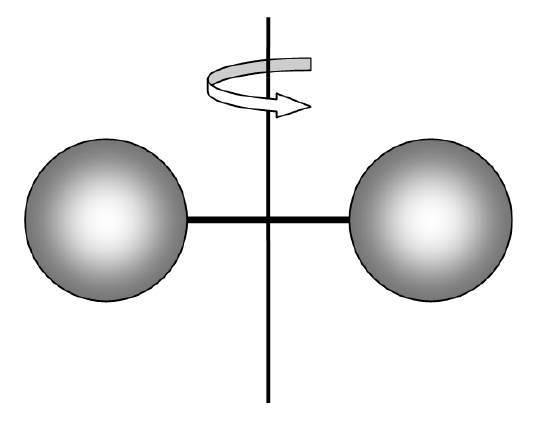
\includegraphics[scale=0.40]{../05_Kruto_tijelo/Zadatak_R302.png}
  \end{center}
  %\caption{Fish}
\end{figure}


